\documentclass[10pt]{article}

\usepackage{adjustbox}
\usepackage{amsmath}
\usepackage[french, onelanguage]{algorithm2e}
\usepackage[utf8]{inputenc}
\usepackage[french]{babel}
\usepackage{csquotes}
\usepackage[T1]{fontenc}
\usepackage{geometry}
\usepackage{glossaries}
\usepackage{graphicx}
\usepackage[hidelinks]{hyperref}
\usepackage[utf8]{inputenc}
\usepackage{listings}
\usepackage{lstautogobble}
\usepackage{tabularx}
\usepackage{textcase}
\usepackage{tikz}
\usepackage{tocloft}
\usepackage{verbatim}
\usepackage{xcolor}
\usepackage{fancyhdr}
%\usepackage[pdf]{pstricks}
%\usepackage{auto-pst-pdf}
%\usepackage{uml}

\makeglossaries

\newacronym{gui}{GUI}{Graphical User Interface}
\newacronym{jdk}{JDK}{Java Development Kit}
\newacronym{ram}{RAM}{Random Access Memory}
\newacronym{json}{JSON}{JavaScript Oriented Notion}
\newacronym{ttmc}{TTMC}{Tu te mets combien?}
\newacronym{po}{PO}{Product Owner}

\usetikzlibrary{calc, shapes.multipart, chains, arrows}

\definecolor{RoyalBlue}{cmyk}{1, 0.50, 0, 0}

\lstset{language=Java,
  keywordstyle=\color{RoyalBlue},
  basicstyle=\scriptsize\ttfamily,
  commentstyle=\ttfamily\itshape\color{darkgray},
  stringstyle=\ttfamily,
  breaklines=true,
  keepspaces=true,
  numbers=left,
  numbersep=5pt,
  showspaces=false,
  showstringspaces=false,
  showtabs=false,
  tabsize=4,
  autogobble=true,
  inputencoding=utf8,
  extendedchars=false,
  backgroundcolor=\color{gray!10},
  texcl=true
}

\geometry{
  a4paper,
  total={170mm,237mm},
  left=20mm,
  top=30mm,
}

\pagestyle{fancy}
\setlength{\headheight}{55.6pt}
\addtolength{\topmargin}{-43.6pt}
\setlength{\footskip}{60pt}
\fancyhf{}
\rhead{
\includegraphics[width=4cm]{header.jpg}}
\rfoot{
\includegraphics[width=4cm]{footer.jpg}}

\begin{document}

\begin{titlepage}
  \centering
  \vspace*{\fill}
  \begin{center}
    \Huge 
    \textbf{What do you know about it? }\\
    \vspace*{0.5cm}
    \large
    \textit{Giorgio Caculli LA196672, Guillaume Lambert LA198116, Tanguy Taminiau LA199566 \\ Groupe B05}
    \vspace*{0.5cm}
    \\ \today
  \end{center}
  \vspace*{\fill}
  \thispagestyle{fancy}
\end{titlepage}	

\newpage
\tableofcontents
\thispagestyle{fancy}

Dans le cadre du cours de ``Projets'' de l'UE 210, nous allons devoir créer un jeu similaire à ``\acrlong{ttmc}'' (\acrshort{ttmc}). L'objectif pédagogique de ce projet est de pousser l'élève a mieux appréhendé la librairie JavaFX vu au cours de 
POO (programmation orienté object). De plus la grande liberté accordé à ce projet consent et oblige l'élève à apprendre à se documenter et savoir faire des recherches.  L'objectif du projet est simple, créer un jeu sur le principe de TTMC (Tu Te 
mets Combien ?).  

\section{Présentation du sujet}
nous allons devoir créer un jeu similaire à TTMC.
Il s'agit d'un jeu comportant des cartes comportant des questions. Il existe quatre thèmes repérable par leurs couleurs respectives, la couleur:
\begin{itemize}
	\item mauve est attribué aux cartes ayant pour thème ``improbable''
	\item orange pour ``plaisir''
	\item bleu pour ``informatique''
	\item vert pour ``scolaire''
\end{itemize}
Chaque carte possède un thème, un sujet en rapport avec le thème, et quatre questions.\\
Les question sont numéroté de un à quatre et triées par ordre croissant de difficulté.
\subsection{Règle du jeu}
Le jeu a pour but de démontrer que l'on se connait mieux que les autres se connaissent eux-même.
Pour le montrer, il faut arriver au bout du plateau tout en gagnant des points.
Pour avancer, il faut répondre correctement aux questions qui se poseront, une bonne réponse nous fait avancer d'une case.
Nous pouvons choisir entre quatres difficultés de questions, en fonction de ce que nous connaissons le mieux. Le niveau 1 est le plus facile et le niveau 4 le plus difficile.
A chaque bonne réponse, nous gagnons un nombre de points équivalant au niveau de la question. Par exemple: nous répondons corretement à une question de niveau 1, nous gagnons 1 point. Si nous répondons correctement à une question de niveau 4, 
nous gagnons 4 points. Lorsqu'un joueur arrive sur la dernière case du plateau, il est désigné gagnant si il est le seul à avoir atteint la fin du plateau ou (si ils sont plusieurs sur la dernière case) si il a le plus de points. 

\subsection{Position du problème}
La création d'un jeu vidéo étant une première pour nous, le problème résidait surtout dans la mamière dont nous allions structuré notre projet mais aussi imaginer se jeu autant dans sa présentation graphique que dans les fonctionnalités a 
incorporé. Les fonctionnalités du jeu nous ont demandé beaucoup de réflexions surtout que nous avions de grande ambition.


Voici l'histoire d'un nain capable de courir vite et de voyager loin.\\
Dans son épopée formidable nous le suivrons une bière à la main.\\


\subsection{Product backlog}
\noindent\adjustbox{max width=\textwidth}{
\begin{tabular}{| p{1cm} | p{16cm} |}
	\hline
	US-01 & En tant qu'utilisateur je voudrais savoir mon score.\\
	\hline
	US-02 & En tant qu'utilisateur je voudrais savoir si j'ai bien répondu.\\
	\hline
	US-03 & En tant qu'utilisateur je voudrais savoir si j'ai mal répondu.\\
	\hline
	US-04 & En tant qu'utilisateur je voudrais savoir quelle était la bonne réponse.\\
	\hline
	US-05 & En tant qu'utilisateur je voudrais savoir mettre mon jeu sur pause.\\
	\hline
	US-06 & En tant qu'utilisateur je voudrais savoir reprendre mon jeu où je l'avait laissé.\\
	\hline
	US-07 & En tant qu'utilisateur je voudrais savoir arrêter mon jeu à tout moment.\\
	\hline
	US-08 & En tant qu'utilisateur j'aimerais joué en multi joueur localement.\\
	\hline
	US-09 & En tant qu'administrateur je dois pouvoir ajouter une nouvelle carte au deck.\\
	\hline
	US-10 & En tant qu'administrateur je veux pouvoir supprimer une carte du deck.\\
	\hline
	US-11 & En tant qu'administrateur je veux pouvoir modifier une carte existante.\\
	\hline
	US-12 & En tant qu'utilisateur j'aimerais avoir une musique de fond.\\
	\hline
	US-13 & En tant qu'utilisateur j'aimerais pouvoir gérer le volume de la musique.\\
	\hline
	US-14 & En tant qu'utilisateur j'aimerais pouvoirs activer ou désactiver la musique de fond.\\
	\hline
	US-15 & En tant qu'utilisateur je voudrais pouvoir choisir mon propre pseudonyme.\\
	\hline
	US-16 & En tant qu'utilisateur je voudrais voir un plateau de jeu.\\
	\hline
	US-17 & En tant qu'utilisateur je voudrais avoir mon pion.\\
	\hline
	US-18 & En tant qu'utilisateur je voudrais savoir reconnaitre mon pion.\\
	\hline
	US-19 & En tant que joueur, je voudrais communiquer avec d'autre joueurs.\\
	\hline
	US-20 & En tant que joueur, j'aimerais jouer avec d'autre joueurs en ligne.\\
	\hline
	US-21 & En tant que joueur, j'aimerais rejoindre une partie en ligne.\\
	\hline
	US-22 & En tant que joueur, j'aimerais héberger une partie en ligne.\\
	\hline
\end{tabular}
}

\subsection{Les classes}

\subsubsection{Le modèle}

\subsubsection{La vue}

\subsubsection{Les exceptions}

\subsection{Explication générale}

\subsection{Diagramme de classe}

\subsection{Extrait de code source}
Voici l'histoire d'un nain capable de courir vite et de voyager loin.\\
Dans son épopée formidable nous le suivrons une bière à la main.\\

\subsection{Launcher}
Le launcher est un logiciel à part entière qui permet à la fois de télécharger JavaFX 11 dépendemment de l'OS utilisé sur le système qui le fait tourner ainsi que de lancer l'application. Le launcher permet donc à n'importe qui de savoir lancer 
notre application tant qu'une version Java 11 au minimum est installé.  
\subsection{Chat en ligne}
Fonctionnalité disponible depuis le jeu en multi joueur en ligne. Chat en ligne permet à plusieurs joueur de communiquer ensemble via un hôte (personne ayant décider d'héberger la partie). Les autres joueur devront rejoindre le jeu de l'hôte. 
Pour le reste cela est un chat dans ce qui a de plus commun, tous les joueurs peuvent envoyer des messages lisible par tous les autres. 
\subsection{Traduction dynamique des menus}
Depuis le menu "setting" (paramètre) il est possible de changer la langue du jeux. En la changeant ainsi qu'en redémarrant le jeu. Le jeu aura changer de langue, tous les boutons des menu seront dès lors traduit dans la langue sélectionné.
Les différentes langues disponible sont 
\begin{itemize}
	\item Anglais (par défaut)
	\item Français
	\item Italien
	\item Japonais
\end{itemize} 

\newpage
\section{Implémentation}
\subsection{Menu principal}
Sur ce menu principal, nous pouvons voir cinq boutons. 
\begin{itemize}
	\item un bouton "play!" permettant d'accéder au menu jouer
	\item un bouton "settings" permettant d'accéder au menu paramètre
	\item un bouton "leave the game" permettant de quitter le jeu une fois que le joueur à confirmer son choix de 
		fermer le jeu.
	\item un bouton "admin panel" permettant d'accéder au menu d'administration une fois le login réussi.
	\item et enfin un boutton " credits" permettant de voir les crédits du jeu.
\end{itemize}

\begin{figure}[h]
	\centering
	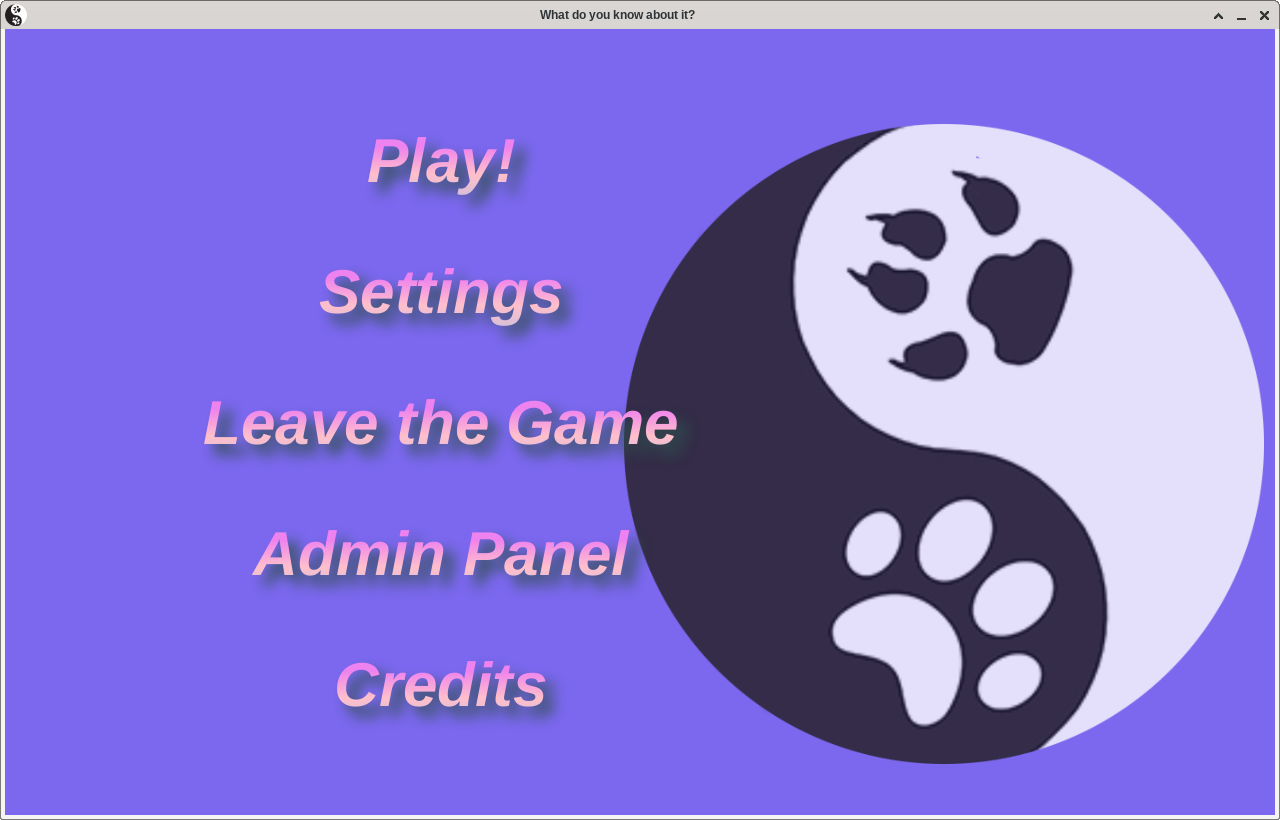
\includegraphics[width=\textwidth]{jeu_main_menu.png}
	\caption{Menu principale du jeu}
	\label{fig:jeu_main_menu}
\end{figure}

\newpage
\subsection{Règle et menu jouer}
Après avoir appuyer sur "Play!", vous arrivez à une fenêtre expliquant les règles du jeu ( celle-ci n'est 
visible que la première fois qu'on appuie sur le boutton "Play!" par lancement de l'application). On accède 
au menu jouer, cette interface possède trois boutons. 
\begin{itemize}
	\item le bouton "Single Player" permettant d'atteindre après avoir mis un pseudo au menu jeu.
	\item le bouton "Multiplayer" permet de parvenir au menu multi joueurs.
	\item le bouton "Return" permet bien evidemment de retourner au menu précédant.
\end{itemize}

\begin{figure}[h]
	\centering
	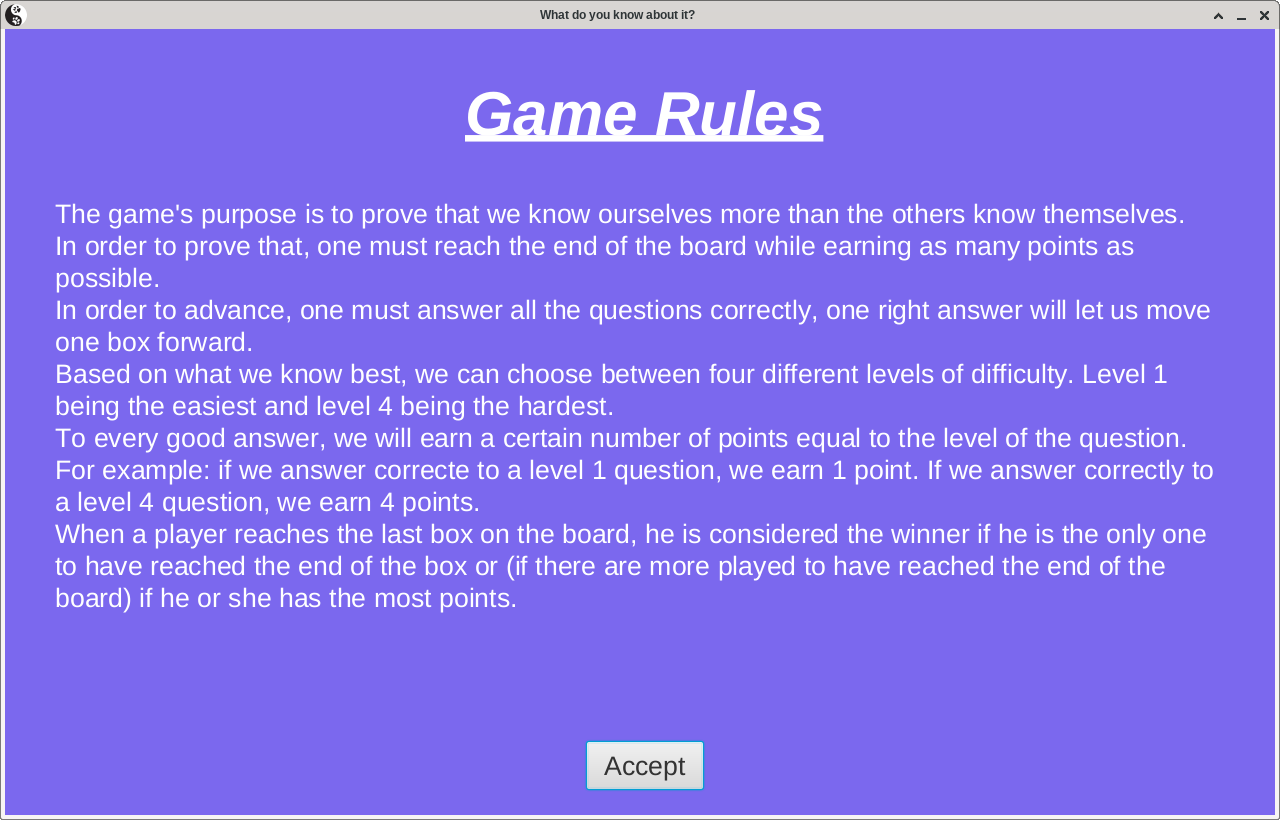
\includegraphics[width=\textwidth]{rule.png}
	\caption{Règle du jeu}
	\label{fig:regle_du_jeu}
\end{figure}

\newpage
\begin{figure}[h]
	\centering
	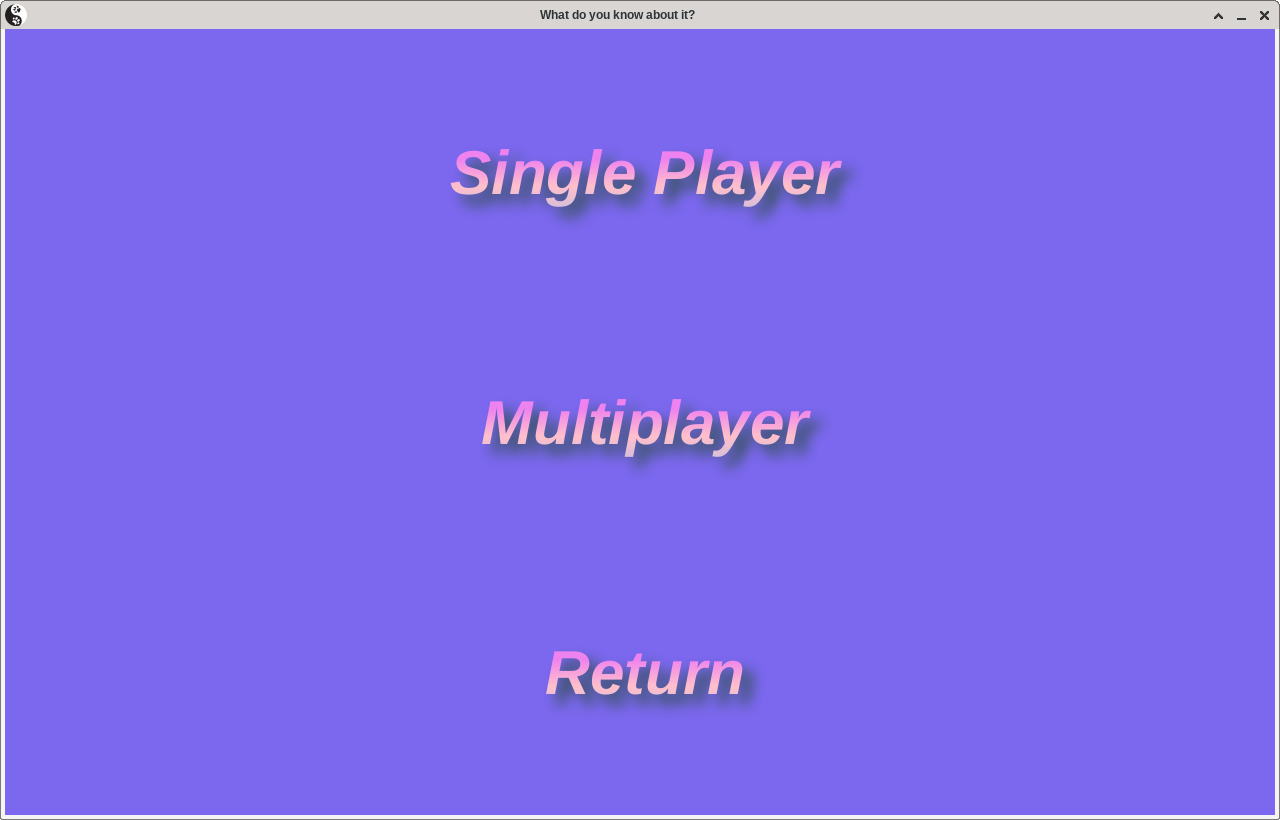
\includegraphics[width=\textwidth]{menujouer.png}
	\caption{menu jouer}
	\label{fig:menu_jouer}
\end{figure}

\newpage
\subsection{Menu jeu}
Menu accessible uniquement en partie solo, ce menu est composé de trois boutons 
\begin{itemize}
	\item Le bouton "New Game" permet de lancer une nouvelle partie.
	\item Le bouton "Load Game" permet de récuperer un deck (fichier json) pour l'utiliser durant la partie.
	\item Le bouton "Return" permet de retourner au menu précédant.
\end{itemize}

\begin{figure}[h]
	\centering
	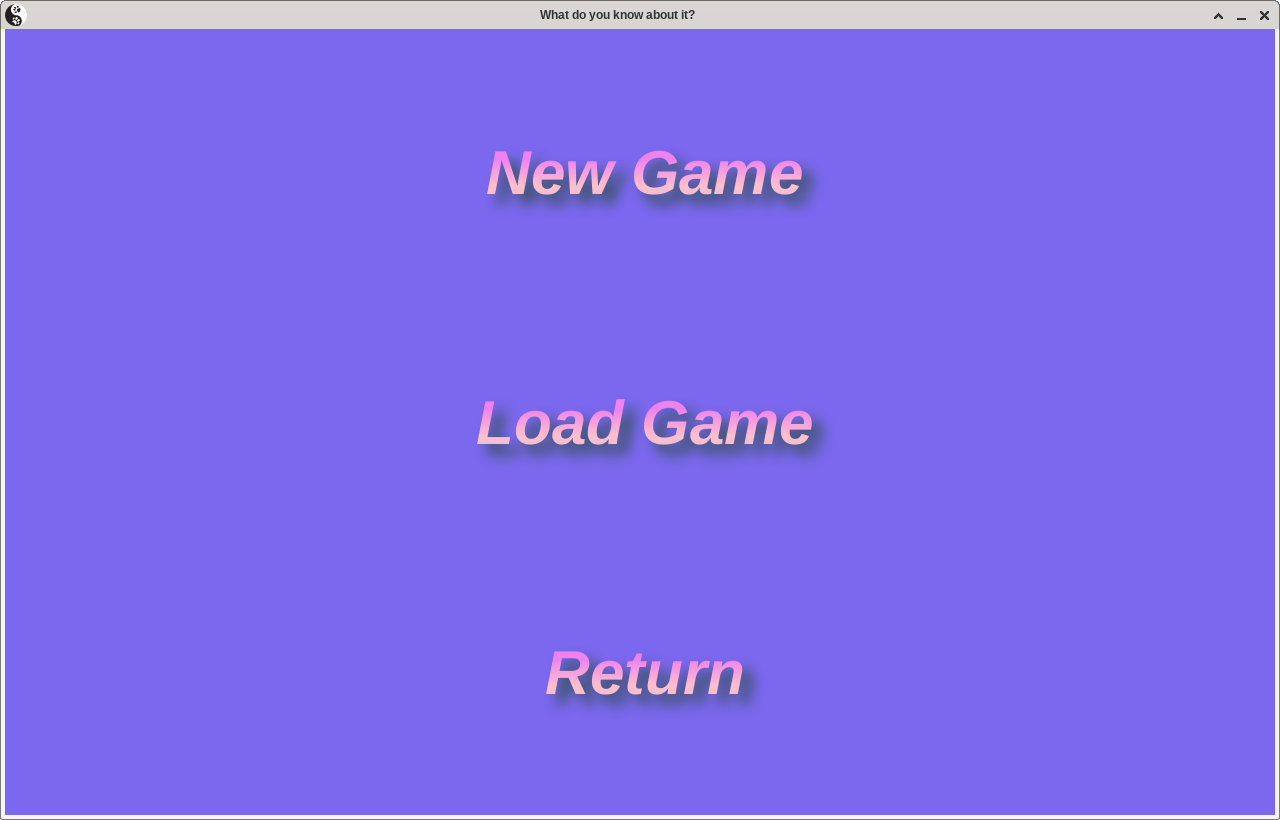
\includegraphics[width=\textwidth]{menujeu.png}
	\caption{menu jeu}
	\label{fig:menu_jeu}
\end{figure}

\newpage
\subsection{Menu multi joueurs}
Dans ce menu, se trouve toute les options disponibles pour les parties multijoueurs. Ce menu est également 
composé de trois boutons.
\begin{itemize}
	\item Un bouton "Local" permet d'accéder à un multi local, il faudra ensuite renseigner le nombre de joueurs
		ainsi que le pseudo de chaque joueur et ensuite appuyer sur "New Game" pour lancer la partie.
	\item Un bouton "Online" permettant d'arriver au menu multijoueur en ligne avec des options propre à se 
		mode de jeu.
	\item le bouton "Return" permet de retourner au menu précédant.
\end{itemize} 

\begin{figure}[h]
	\centering
	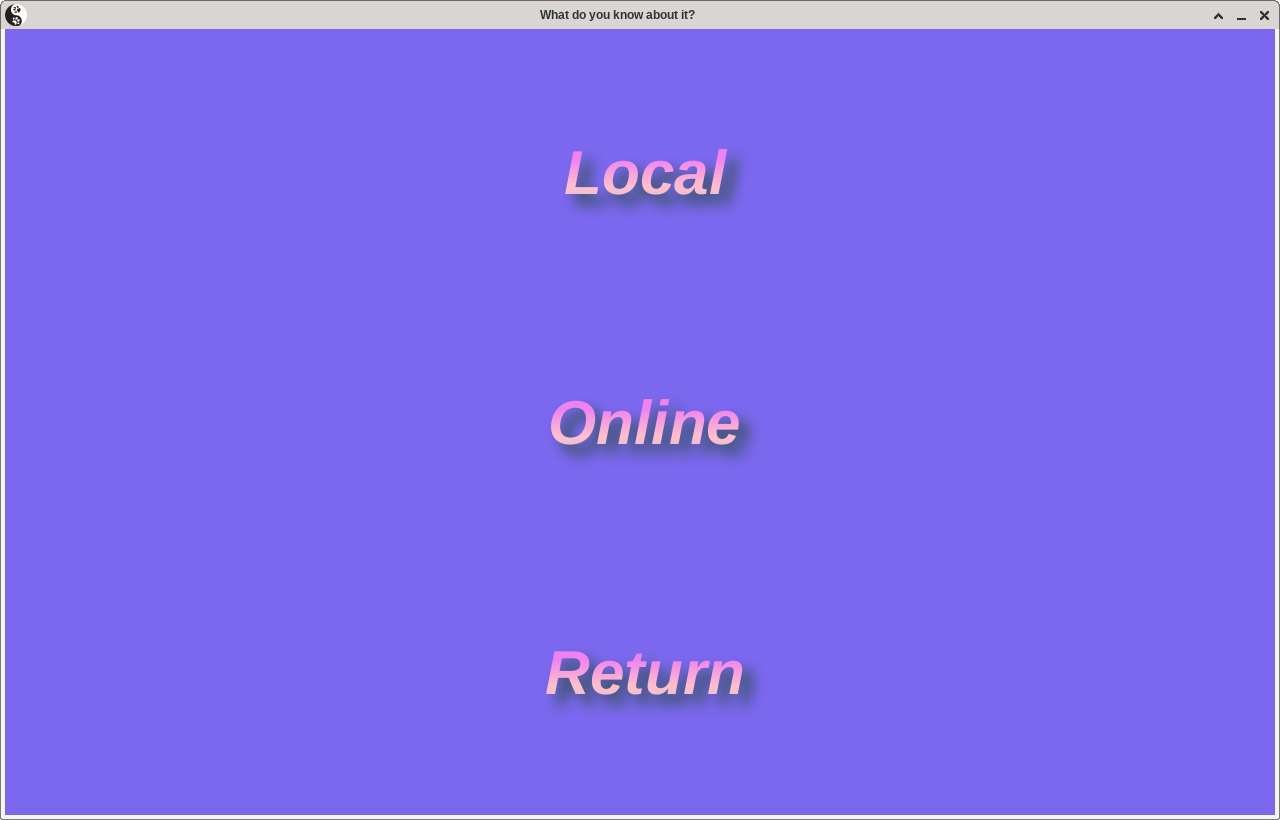
\includegraphics[width=\textwidth]{menumulti.png}
	\caption{menu multi joueurs}
	\label{fig:menu_multi_joueurs}
\end{figure}

\newpage
\subsection{Menu multi joueur en ligne}
Dans ce menu nous retrouverons les options pour le multi en ligne. Ce menu est composé de trois boutons.
\begin{itemize}
	\item Le bouton "Host" permettant d'héberger le jeux.
	\item Le bouton "Join" nous offre la possibilité de rejoindre un joueur hôte. Pour ce faire, après avoir 
		sélectionné cette option, il sera nécessaire de renseigner dans une boite de dialogue  un nom 
		d'utilisateur ainsi que l'adresse IP du joueur hôte.
	\item le bouton "Return" permet de retourner au menu précédant.
\end{itemize}

\begin{figure}[h]
	\centering
	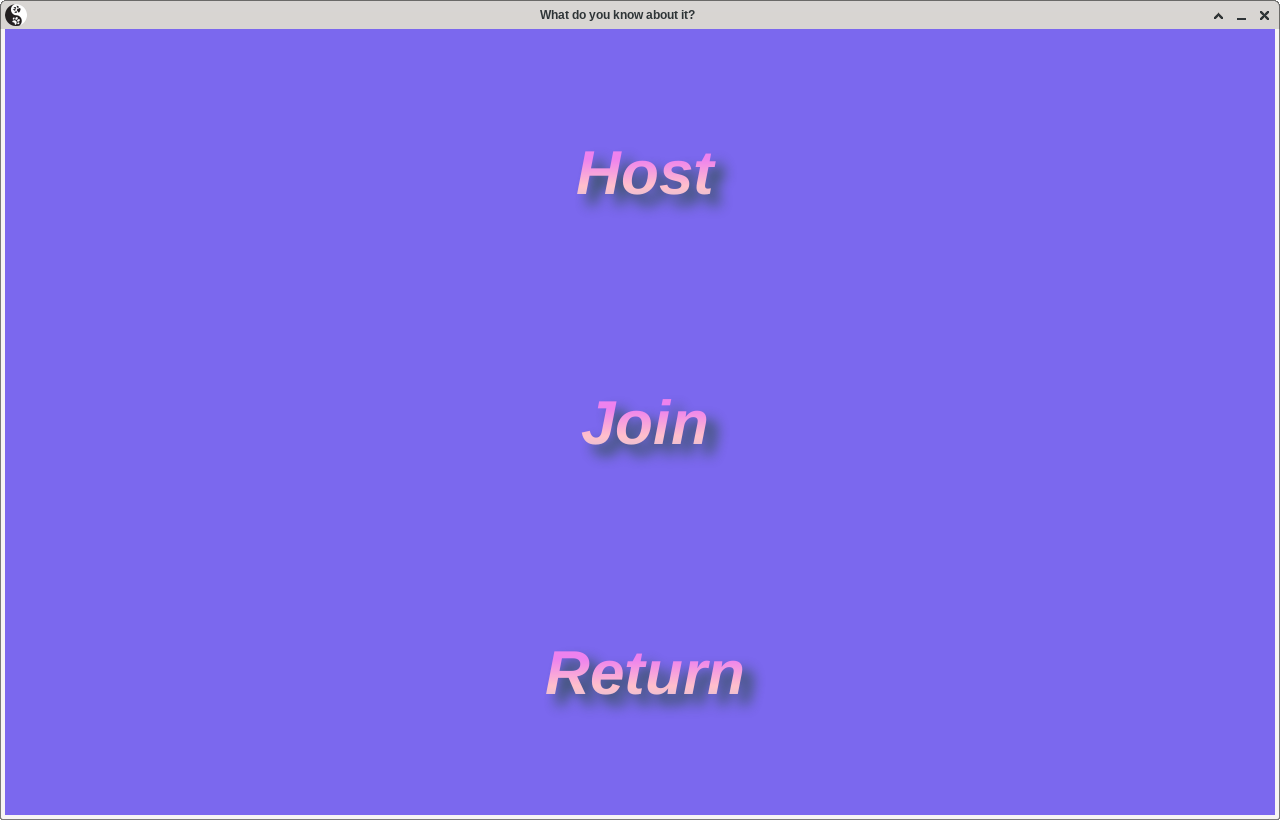
\includegraphics[width=\textwidth]{menuonline.png}
	\caption{menu multi joueur en ligne}
	\label{fig:menu_multi_en_ligne}
\end{figure}

\newpage
\subsection{Menu paramètre}
Ici vous retrouverez tous les options de notre application. Commençons par la barre de volume permettant de gérer 
le volume du son. Cette barre est accompagné d'un bouton "Mute" permettant de complètement mettre le son en 
sourdine. Ensuite ce trouve une textfield permettant de modifier le chrono du jeu. Pour selectionner une langue,
cela se fait depuis une liste déroulante. Les langues disponible sont l'anglais, le français, l'italien et le 
japonais. Vient ensuite une deuxième liste déroulante qui permet cette fois-ci de modifier la taille de la fênetre. Les taille disponible sont 1280x800 et 1440x900. Il est également possible de mettre le jeu en mode plein écran, pour ce faire, il faut cocher l'option "Maximize window".

\begin{figure}[h]
	\centering
	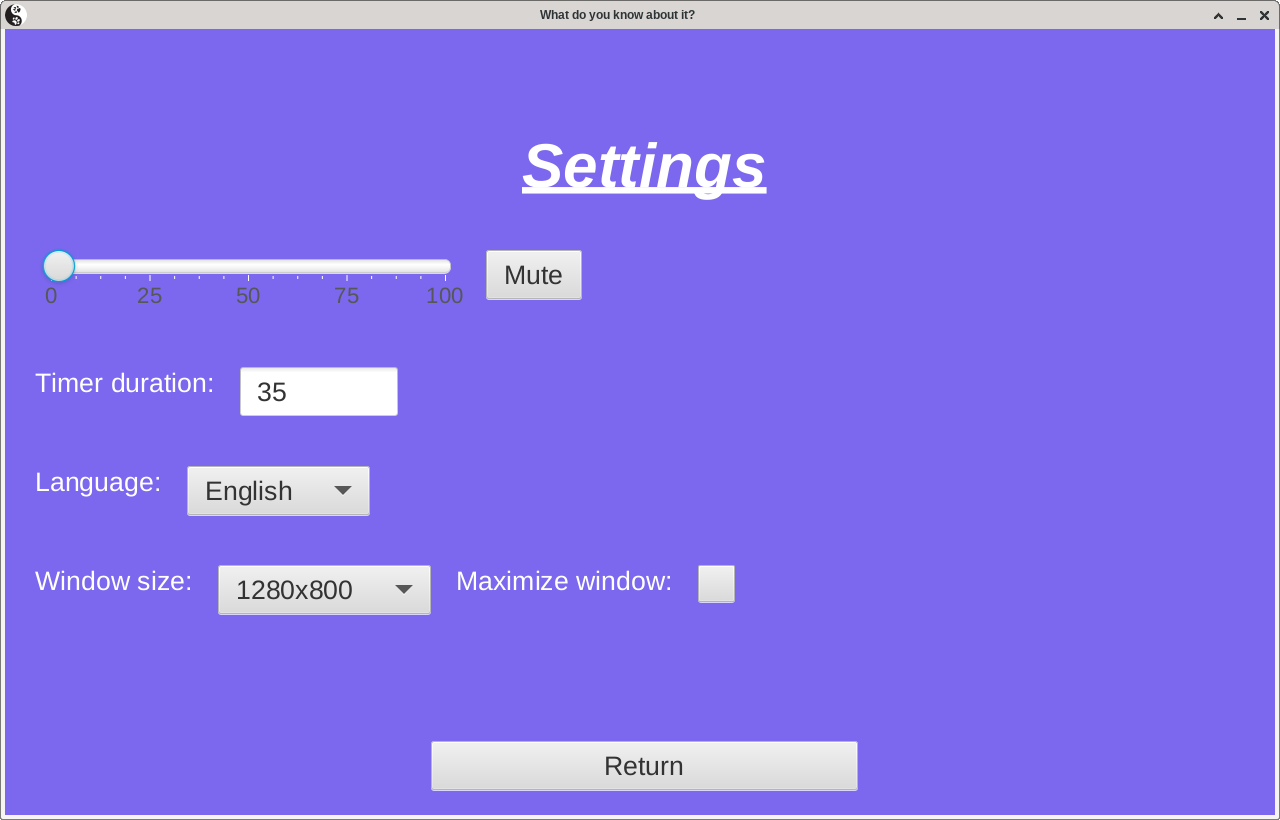
\includegraphics[width=\textwidth]{setting.png}
	\caption{menu paramètre}
	\label{fig:menu_setting}
\end{figure}

\newpage
\subsection{Menu d'administration}
Après avoir cliqué sur le bouton "Admin Panel" du menu principal et vous êtes correctement connecté en tant 
qu'administrateur, vous accéderez au menu administrateur. ce menu est composé de cinq boutons.
\begin{itemize}
	\item Le bouton "Add a new card" permet d'arriver à une nouvelle interface permettant de créer une nouvelle carte.
	\item Le bouton "List of cards" permet d'accèder au tableau de toutes les cartes du deck. Il est également possible de modifier une carte depuis ce tableau
	\item Le bouton "Import a new deck" permet d'importer un nouveau deck pour le jeu. Ce bouton ouvre un explorateur de fichier afin de pouvoir trouver la cible à importer.
	\item Le bouton "Export the current deck" permet d'exporter le deck actuellement utiliser par le jeu. Ce bouton ouvre également un explorateur de fichier afin de pouvoir nommer et placer où on le désire le deck.
	\item le bouton "Return" permet de retourner au menu précédant.
\end{itemize}

\begin{figure}[h]
	\centering
	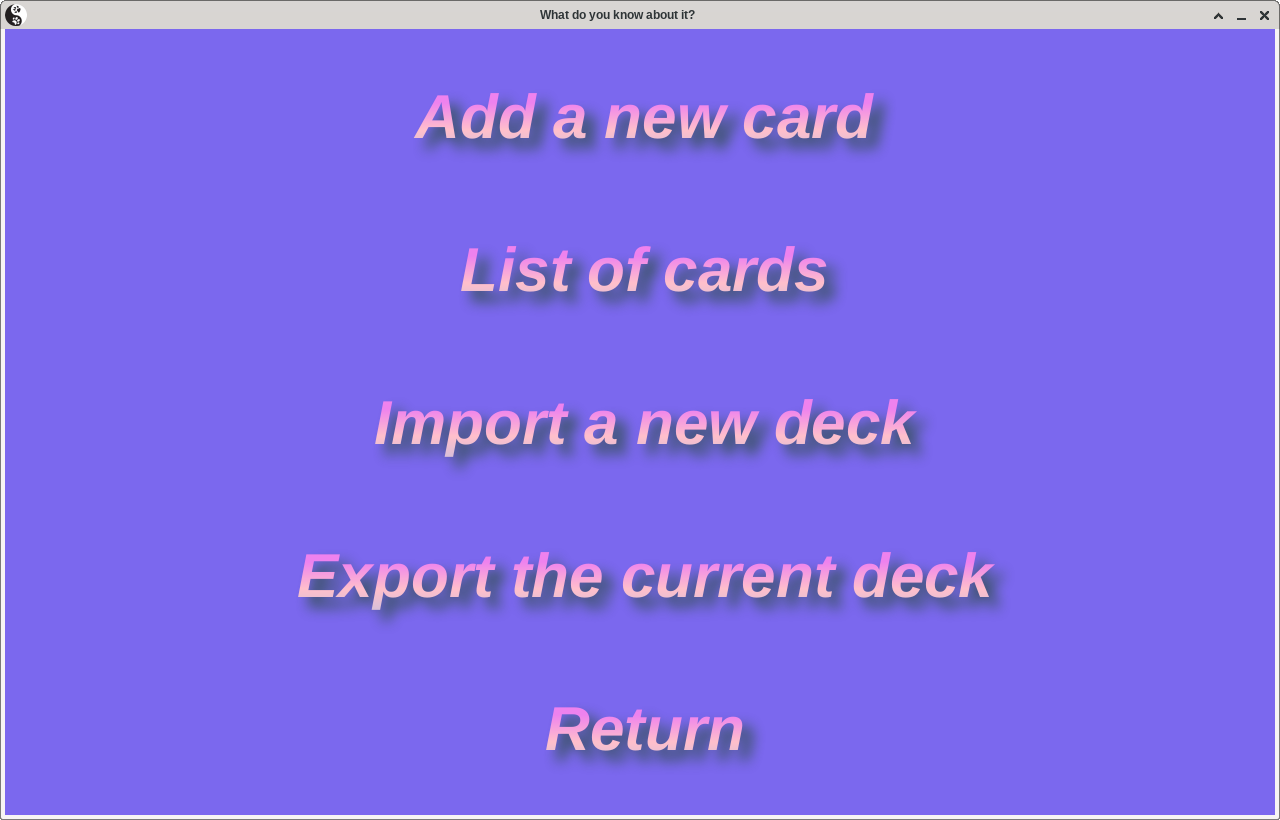
\includegraphics[width=\textwidth]{admin.png}
	\caption{Menu d' administration}
	\label{fig:menu_administration}
\end{figure}

\newpage
\subsection{interface "New Card"}
Cette interface permet d'ajouter une carte au deck. Pour ce faire il faudra d'abord choisir un thème via la 
liste déroulante. Il faudra ensuite renseigner l'auteur, le sujet , les quatres challenge ainsi que les 
quatres réponses. Sachant que le challenge n°1 est le plus facile et donc le challenge 4 est le plus dur.
Le bouton "Add" ajoutera la carte ainsi créé si toute les informations sont bien renseigner. Le bouton "Clean" permet de vider tous les textfields.

\begin{figure}[h]
	\centering
	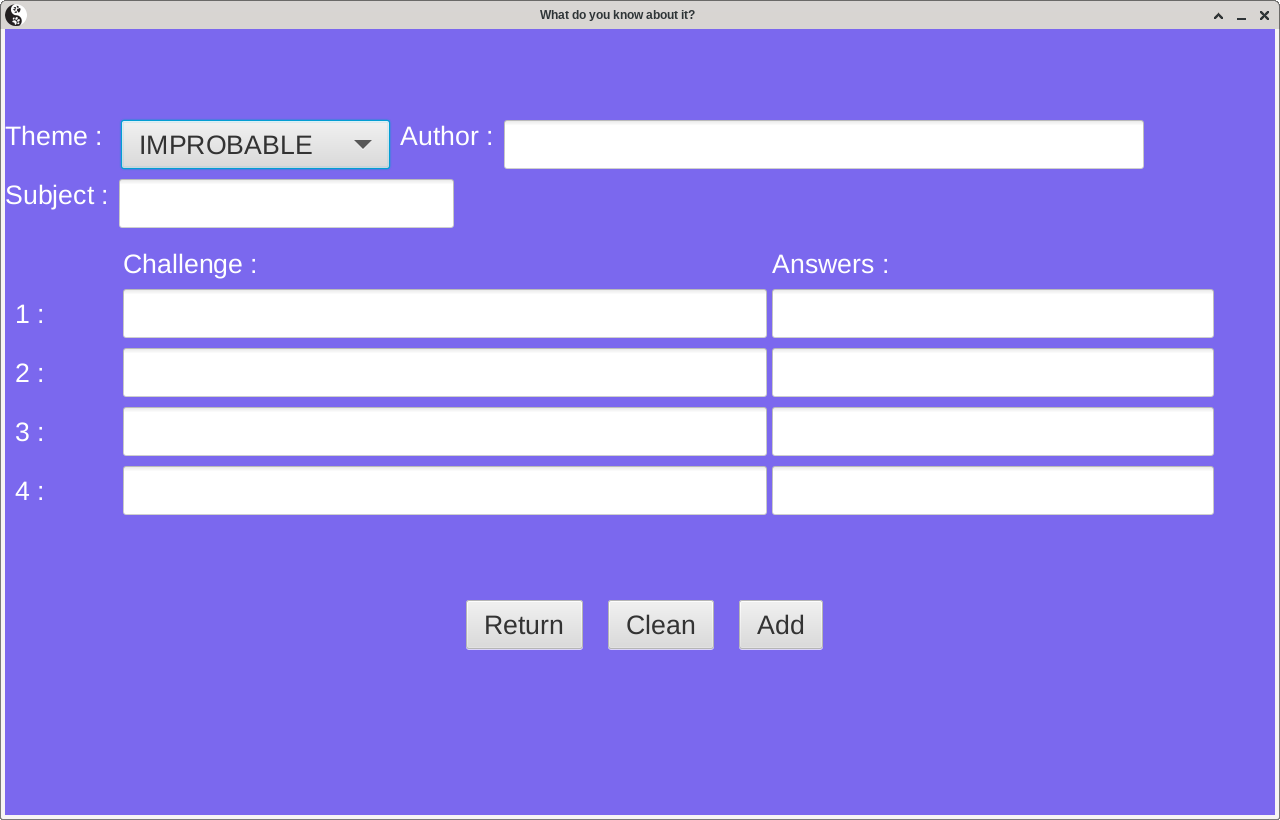
\includegraphics[width=\textwidth]{newcard.png}
	\caption{interface "New card"}
	\label{fig:new_card}
\end{figure}

\newpage
\subsection{Tableau carte}
Cette interface est composé d'un grand tableau de trois colonnes ( auteur, thème et sujet) ainsi que de trois 
boutons. Un bouton "return", un bouton "Reload" permettant de recharger les informations modifier et un bouton 
delete permet à partir d'une sélection de carte de supprimer la carte sélectionné. En double cliquant sur une 
ligne , nous accédons à une interface similaire à "Menu d'administration" si ce n'est que toutes les 
textfields sont déjà rempli. Il ne reste plus qu'à faire les modifications puis appuyer sur" Modify" puis sur "
reload" et toutes les informations ont été mises à jour.

\begin{figure}[h]
	\centering
	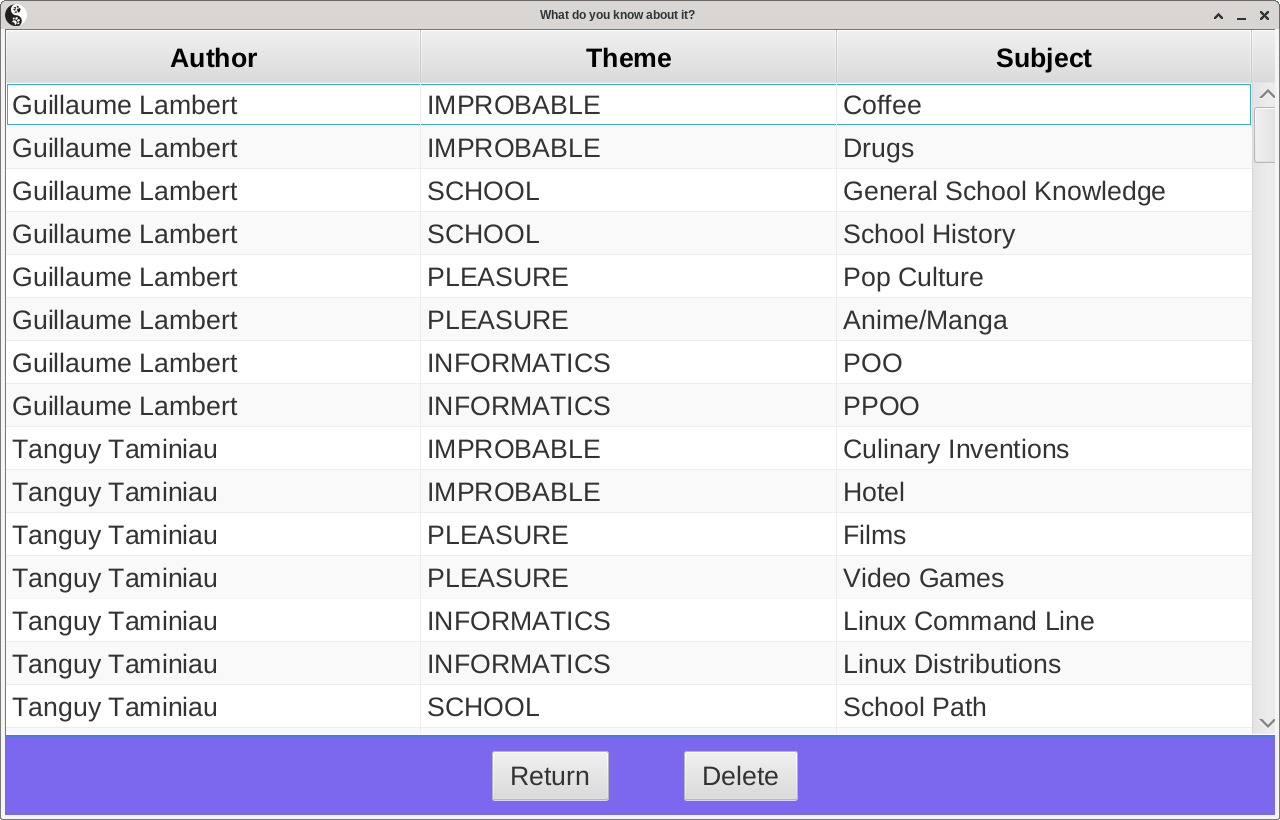
\includegraphics[width=\textwidth]{tablecard.png}
	\caption{Tableau carte}
	\label{fig:tablecard}
\end{figure}


\newpage
\section{Tests unitaires}

Le code présent ci-dessous est celui de la fonction qui permet de rajouter une nouvelle question au deck.
Différent cas de vérification ont lieu avant de permettre à une question quelconque d'être rajoutée.
Le premier cas sert à vérifier que l'objet en entrée ne soit pas null, si c'est le cas, alors la fonction renverra false.
Le deuxième consiste à vérifier que l'ajout ne cause pas de doublon, si c'est le cas, l'exception QuestionDoubleException sera appelée, et false sera renvoyé comme résultat.
Le troisième cas consiste à vérifier que le thème de la question correspond bien à celui de la carte, si c'est pas le cas, QuestionIncompatibleException sera appelée et false sera renvoyé comme résultat.
Le dernier cas de vérification consiste à vérifier qu'il n'y ait pas plus que le nombre maximal de question sur une carte, dans le cas de notre jeu ce dernier équivaut à 4.
Si une 5\up{ème} est rajoutée, l'exception BasicCardOverMaxQuestionsException sera appelée et le résultat sera false;
Si tous les cas de vérifications sont réussis, alors la fonction va ajouter la nouvelle question à la carte, et le résultat sera true.

\begin{lstlisting}
/**
 * Function used to add a new question to the card
 * 
 * @param q The question that the user wishes to add to his card
 * 
 * @return true if added, false if not
 */
public boolean add( Question q )
{
    try
    {
        if ( q == null )
        {
            throw new NullPointerException();
        }
        if ( questions.contains( q ) )
        {
            throw new QuestionDoubleException();
        }
        if ( q.getTheme() != theme || !q.getAuthor().equalsIgnoreCase( author )
                || !q.getSubject().equalsIgnoreCase( subject ) )
        {
            throw new QuestionIncompatibleException();
        }
        if ( questions.size() == 4 )
        {
            throw new BasicCardOverMaxQuestionsException();
        }
        return questions.add( q.clone() );
    }
    catch ( NullPointerException npe )
    {
        npe.printStackTrace();
        return false;
    }
    catch ( QuestionDoubleException qde )
    {
        qde.printStackTrace();
        return false;
    }
    catch ( QuestionIncompatibleException qie )
    {
        qie.printStackTrace();
        return false;
    }
    catch ( BasicCardOverMaxQuestionsException bcomqe )
    {
        bcomqe.printStackTrace();
        return false;
    }
}
\end{lstlisting}

Dans les tests unitaires, cette fonction est vérifiée en lui injectant les différents cas possibles.
Voici une partie du code des tests unitaires qui ont lieu sur BasicCard, ici on ne vérifie que les différentes interactions avec la fonction ``add'' et on s'assure que les différents cas de vérifications soient bien respéctés.

\begin{lstlisting}
public class BasicCardTests
{
    private static BasicCard c1, c2;
    private static Question q1, q2, q3, q4, q5, q6, q7, q8, q9, q10, q11, q12;

    @BeforeAll
    static void initAll()
    {
        c1 = new BasicCard( "Giorgio Caculli", Theme.INFORMATICS, "Acronyms" );
        c2 = c1.clone();
        q1 = new Question( "Giorgio Caculli", Theme.INFORMATICS, "Acronyms", "What does RAM stand for?",
                "Random Access Memory" );
        q2 = new Question( "Giorgio Caculli", Theme.INFORMATICS, "Acronyms", "What does JAR stand for?",
                "Java ARchive" );
        q3 = new Question( "Giorgio Caculli", Theme.INFORMATICS, "Acronyms", "What does WWW stand for?",
                "World Wide Web" );
        q4 = new Question( "Giorgio Caculli", Theme.INFORMATICS, "Acronyms", "What does CPU stand for?",
                "Central Processing Unit" );
        q5 = new Question( "Giorgio Caculli", Theme.INFORMATICS, "Acronyms", "What does GPU stand for?",
                "Graphics Processing Unit" );
        q6 = new Question( "Giorgio Lambert", Theme.INFORMATICS, "Acronyms", "What does IT stand for?",
                "Information Technology" );
        q7 = new Question( "Giorgio Caculli", Theme.IMPROBABLE, "Acronyms", "What does IT stand for?",
                "Information Technology" );
        q8 = new Question( "Giorgio Caculli", Theme.INFORMATICS, "Acronym", "What does IT stand for?",
                "Information Technology" );
        q9 = q5.clone();
        q10 = new Question( "Giorgio Caculli", Theme.INFORMATICS, "Acronyms", "What does JDK stand for?",
                "Java Development Kit" );
        q11 = new Question( "Giorgio Caculli", Theme.INFORMATICS, "Acronyms", "What does OOP stand for?",
                "Object Oriented Programming" );
        q12 = new Question( "Giorgio Caculli", Theme.INFORMATICS, "Acronyms", "What does OS stand for?",
                "Operating System" );
    }

    @BeforeEach
    void init()
    {
    }

    @Test
    public void testAddQuestions()
    {
        assertTrue( () -> c1.add( q1 ), "failure - the question was not added" );
        assertTrue( () -> c1.add( q2 ), "failure - the question was not added" );
        assertTrue( () -> c1.add( q3 ), "failure - the question was not added" );
        assertTrue( () -> c1.add( q4 ), "failure - the question was not added" );
    }

    @Test
    public void testAddDouble()
    {
        assertFalse( () -> c1.add( q1 ), "failure - the question was added" );
    }

    @Test
    public void testAddMoreThanFourQuestions()
    {
        assertTrue( () -> c1.add( q11 ), "failure - the question was not added" );
        assertFalse( () -> c1.add( q12 ), "failure - the question was added" );
    }

    @Test
    public void testAddQuestionWithDifferentAuthor()
    {
        assertFalse( () -> c1.add( q6 ), "failure - the question was added" );
    }

    @Test
    public void testAddQuestionWithDifferentTheme()
    {
        assertFalse( () -> c1.add( q7 ), "failure - the question was added" );
    }

    @Test
    public void testAddQuestionWithDifferentSubject()
    {
        assertFalse( () -> c1.add( q8 ), "failure - the question was added" );
    }

    @Test
    public void testAddNullQuestion()
    {
        assertFalse( () -> c1.add( null ), "failure - the question was added" );
    }
}
\end{lstlisting}

Voici le rapport de couverture des différents tests menés sur les différentes fonctions de BasicCard

\begin{figure}[h]
	\centering
	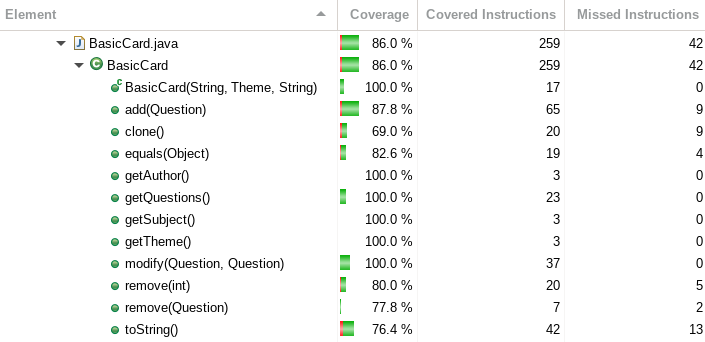
\includegraphics[width=\textwidth]{junit_coverage.png}
	\caption{Rapport de couverture du code}
	\label{fig:diag_coverage}
\end{figure}



\section{Conduite du projet}
Voici l'histoire d'un nain capable de courir vite et de voyager loin.\\
Dans son épopée formidable nous le suivrons une bière à la main.\\


\section{Conclusion}
Voici l'histoire d'un nain capable de courir vite et de voyager loin.\\
Dans son épopée formidable nous le suivrons une bière à la main.\\


\newpage
\printglossary

\end{document}
